\documentclass{article}[12pt]
\usepackage{enumitem}
\usepackage{hyperref}
\usepackage{xcolor}
\usepackage[T1]{fontenc} % Should be Times New Roman adjacent, from https://tex.stackexchange.com/questions/33677/setting-font-family-for-the-whole-document
\usepackage{mathptmx}
\usepackage{moresize}
\usepackage{setspace}
\usepackage{float} 
\usepackage{placeins}
\usepackage{ntheorem}
\usepackage{amsmath}
\usepackage{amssymb}
\usepackage{mathtools}
\usepackage[separate-uncertainty = true]{siunitx}
\usepackage[framemethod=tikz]{mdframed}
\usepackage{graphicx}
\usepackage{cancel}
\usepackage{multicol}
\usepackage[margin=2.5cm]{geometry}
\usepackage{listings}
\graphicspath{ {./images/} }
\pdfoutput=1
\onehalfspacing

\nonstopmode

\hypersetup{
    colorlinks,
    linkcolor={black!100!black},
    urlcolor={black!100!black}
}

\sisetup{
    number-unit-product=~
    } % Taken from M\X's answer on https://tex.stackexchange.com/questions/160105/unit-spacing-with-siunitx-in-an-equation

\newcommand{\uhref}[2]{\href{#1}{\underline{#2}}} % For directly linking to websites.
\newcommand{\reference}[3]{(#2, #3)\textsuperscript{\ref{#1}}} % For doing Harvard style referencing. Label should go at the bottom, reference at value being referenced.
\newcommand{\thlineA}{\hline ~ & ~ & ~ & ~ & ~ \\[-2ex] } % The values in the table get squished when using the regular hline, this adds a small bit of extra space at the top by adding a phantom row with negative bottom spacing.
\newcommand{\thline}{\hline ~ & ~ & ~ & ~ \\[-2ex] }


\begin{document}
    %Cover Page, centers text in middle of page
    \vspace*{\fill}
    \hrule
    \vspace*{10pt}
    \begin{center}
            \huge\textbf{Determining Planck's Constant} \\
            DRAFT - NOT FINAL SUBMISSION \\
            \Large Daire O'Brien - 24365676 \\
            \large Department Of Physics, \\
            Maynooth University \\ ~ \\
            Thanks to \\
            Adam O'Connor - Lab partner\\
            Milosz Wegorski - Demonstrator\\~\\
            \normalsize 
            Experiment conducted: November 10, 2025 \\
            Document compiled: \today \\
    \end{center}
    \vspace*{10pt}
    \hrule
    \vspace*{\fill}
    %Prevents the cover page from having a page number on it
    \setcounter{page}{0}
    \pagenumbering{gobble}
    \newpage
    \pagenumbering{arabic}
    \setcounter{page}{1}
    \tableofcontents
    \addcontentsline{toc}{section}{Abstract}
    \section*{Abstract}
        The value of Planck's Constant $h$ was measured by analysing the voltage generated when photons of differing wavelenghts strike a caesium cathode. The value of $\qty{6.55(0.387)E-34}{\J\per\H}$ was found, which agrees with the defined value of $\qty{6.62607015E-34}{\J\per\H}$ \reference{reference:plancksConstant}{NIST}{2022}. 
    \newpage
    \section{Introduction}
        \subsection{Background}
            In 1887 physicist Heinrich Hertz noticed that exposing a spark gap to UV light would increase the maximum lengh \reference{reference:uvPaper}{Hertz, Heinrich}{1887}
        \subsection{Theory}

    \section{Experiment}
        \subsection{Apparatus}
            \begin{itemize}
                \item 3B Scientific Planck's Constant Apparatus 1000537 / U10700-230 \reference{reference:apparatusDocumentation}{3B Scientific}{2024} \\
                Within the supplied apparatus is a 
                \begin{itemize}
                    \item 1P39 Photoelectric Tube
                    \item Voltmeter
                    \item Nanoammeter
                    \item LED power supply
                \end{itemize}
                \item LEDs of wavelenghts
                \begin{itemize}
                    \item $\qty{472}{\nm}$
                    \item $\qty{505}{\nm}$
                    \item $\qty{525}{\nm}$
                    \item $\qty{588}{\nm}$
                    \item $\qty{611}{\nm}$
                \end{itemize}
            \end{itemize}
        \subsection{Method}
            \begin{figure}[!h]
                \centering
                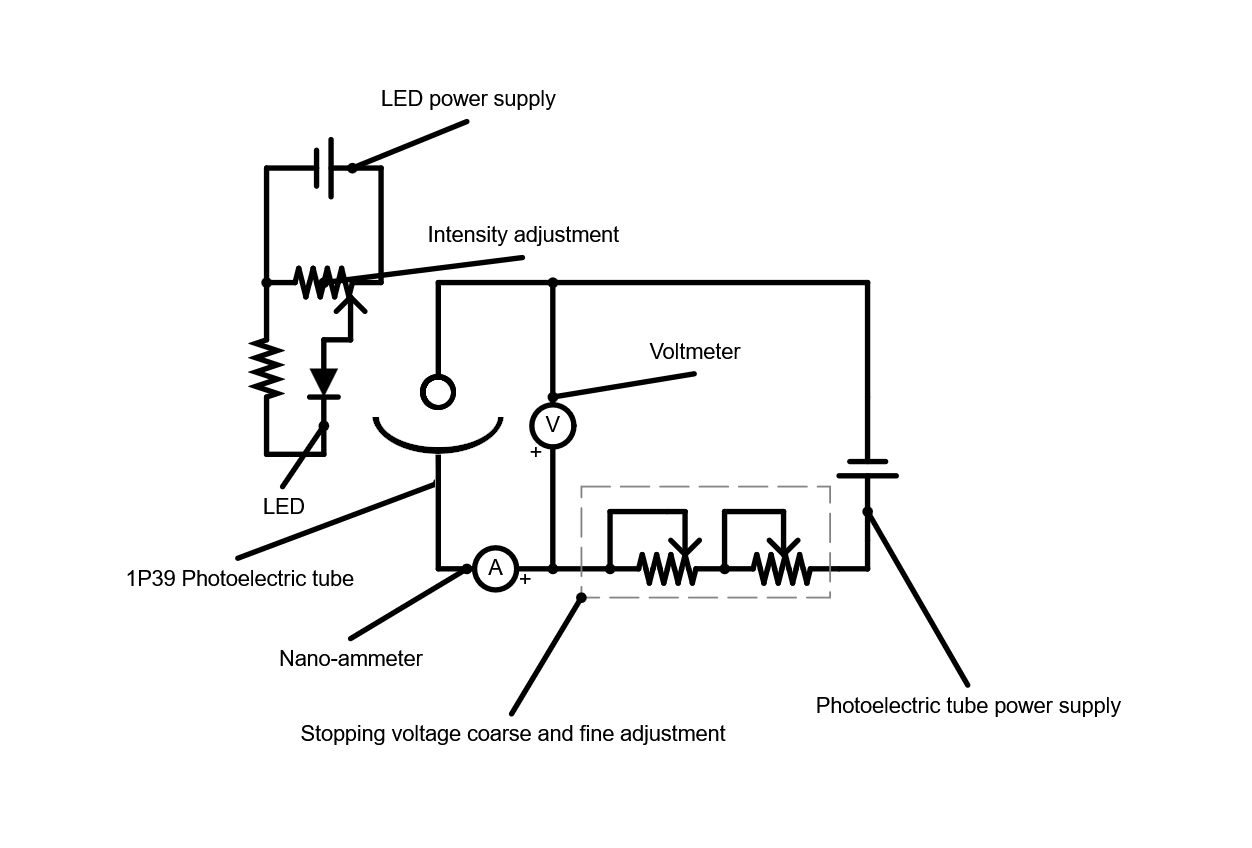
\includegraphics[width=0.8\textwidth]{CircuitDiagram2}
                \caption{Diagram for the internal circuitry of the apparatus}\label{circuitdiagram}
            \end{figure}
            \subsubsection{Part 1}
                The equipment was set up as shown in figure \ref{circuitdiagram}. The apparatus was connected to mains voltage. The LED's power connector was plugged in and the output secured onto the plastic cover surrounding the photoelectric tube. The intensity was set to $75\%$. The LED was turned on. The setup was then allowed to stabelize for 1 minute. The coarse adjustment knob was turned until the reading on the nano-ammeter was approximately $\qty{0}{\A}$. The fine adjustment knob was then turned until the nano-ammeter oscillated between $-\qty{0}{\A}$ and $+\qty{0}{\A}$, where the critical voltage roughly equaled the back-emf generated by the photoelectric tube. The value on the voltmeter was then recorded. This was repeated for all 5 LEDs.
            \subsubsection{Part 2}
                The equipment was set up as shown in figure \ref{circuitdiagram}. The apparatus was connected to mains voltage. The LED's power connector was plugged in and the output secured onto the plastic cover surrounding the photoelectric tube. The intensity was set to $100\%$. Using the adjustment knobs, the stopping voltage was adjusted until the nano-ammeter oscillated between $-\qty{0}{\A}$ and $+\qty{0}{\A}$. The voltage was recorded. This was repeated 5 times, each time reducing the intensity by $20\%$. The LED was then changed for one of a different wavelenght. This was done for the $\qty{472}{\nm}$, $\qty{525}{\nm}$ and $\qty{611}{\nm}$ LEDs.
    \FloatBarrier
    \section{Results}
        \begin{table}[!h]
            \centering
            \begin{tabular}[center]{|c|c|c|c|}
                \hline
                Name & Symbol & Value & Reference \\
                \thline
                Electron charge & $e$ & $\qty{1.602E-19}{\C}$ & \reference{reference:electronCharge}{NIST}{2022} \\
                \thline
                Speed of light in a vacuum & $c$ & $\qty{2.998E8}{\m\per\s}$ & \reference{reference:speedOfLight}{BIPM}{2019} \\
                \thline
                Accepted value of Planck's constant & $h$ & $\qty{6.626E-34}{\J\per\H}$ & \reference{reference:plancksConstant}{NIST}{2022} \\
                \thline 
                Accepted value of the Work function of caesium & $w$ & $\qty{1.95}{\eV}$ & \reference{reference:workFunction}{Lide, D.R.}{2008} \\
                \hline
            \end{tabular}
            \caption{Constants and accepted values}\label{constants}
        \end{table}
        \subsection{Part 1}
            {\small
            \begin{table}[!h]
                \centering
                \begin{tabular}[center]{|c|c|c|c|c|}
                \thlineA
                Wavelength $[\unit{\nm}]$ & Wavelenght $[\unit{\m}]$  & $V_0 ~ [\unit{\V}]$ & Energies $eV_0 ~ [\unit J]$ & Frequencies $[\unit{\Hz}]$\\
                \thlineA
                $472$ & $\num{4.14E-7}$ & $0.663$ & $\num{1.062E-19}$ & $\num{6.36E14}$ \\
                \thlineA
                $505$ & $\num{5.05E-7}$  & $0.514$ & $\num{8.23E-20}$ & $\num{5.94E14}$\\
                \thlineA
                $525$ & $\num{5.25E-7}$  & $0.465$ & $\num{7.45E-20}$ & $\num{5.71E14}$\\
                \thlineA
                $588$ & $\num{5.88E-7}$  & $0.161$ & $\num{2.58E-20}$ & $\num{5.10E14}$\\
                \thlineA
                $611$ & $\num{6.11E-7}$  & $0.085$ & $\num{1.36E-20}$ & $\num{4.91E14}$\\
                \hline
            \end{tabular}
            \caption{Energies and frequencies for the photons}\label{wavelenghts}
            \end{table}}
            \normalsize
            Each of the energies were taken as 
                \begin{equation}\label{EnergyEquation}
                    E = eV_0
                \end{equation}
            Where $e$ is the charge of an electron. The frequencies were taken as
                \begin{equation}\label{FrequencyEquation}
                    f = \frac {c}{\lambda}
                \end{equation}
            Where 
            {\begin{figure}[!h]
                \centering
                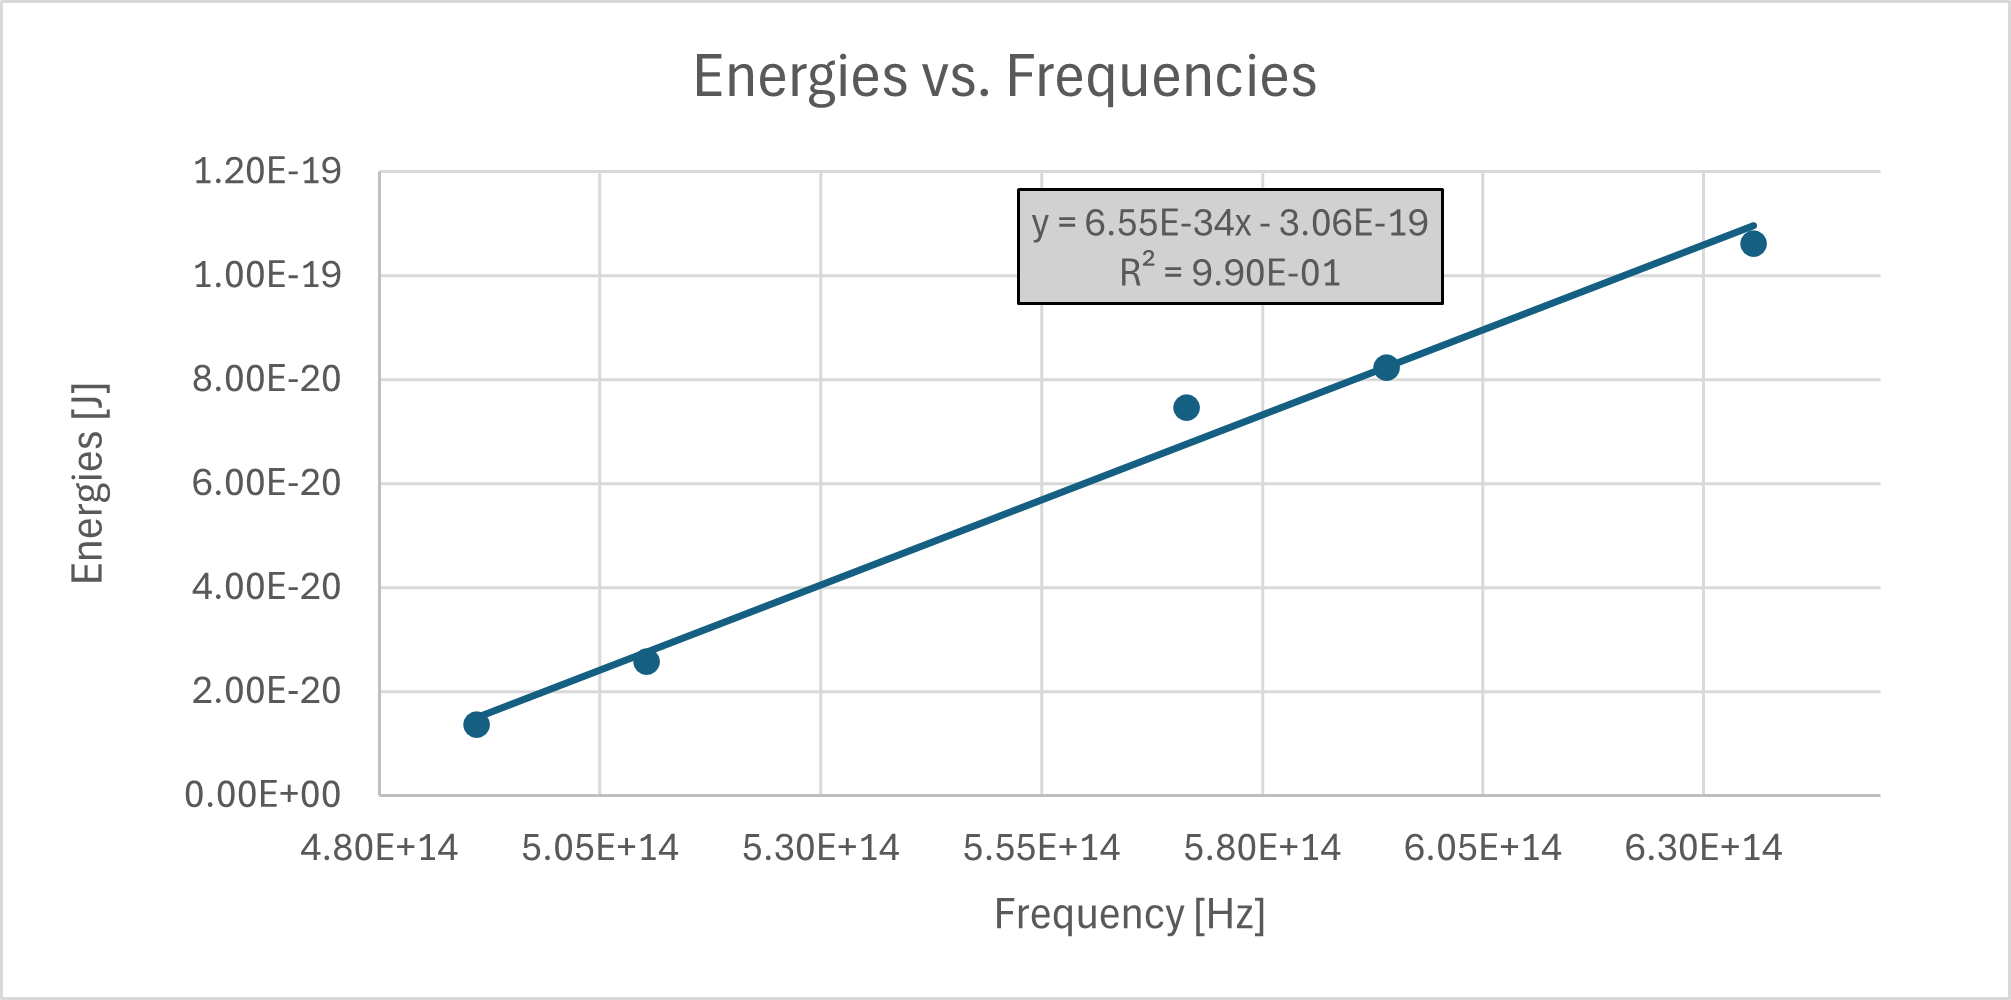
\includegraphics[width=0.8\textwidth]{EnergiesvsFrequencies}
                \caption{Graph of the energies and frequencies from table \ref{wavelenghts}}\label{EnergiesvsFrequenciesGraph}
            \end{figure}}


            {\small \begin{table}[!h]
                \centering
                \begin{tabular}[center]{|c|c||c|c|}
                    \thline
                    $h \ [\unit{\J\per\H}]$ & $\num{6.54E-34}$ & Constant $[\unit{\J}]$ & $\num{-3.06E-19}$ \\ \thline
                    $\Delta h \ [\unit{\J\per\H}]$ & $\num{3.9E-35}$ & $\Delta \text{Constant }[\unit{\J}]$ & $\num{2.17E-20}$ \\
                    \thline
                    $r^2$ & $0.989$ & $\Delta y$ [J] & $\num{4.6E-21}$ \\
                    \thline
                    F statistic & $\num{287.1}$ & Degrees of freedom & $\num{3}$ \\
                    \thline 
                    ssreg & $\num{6.102E-39}$ & ssresid & $\num{6.376E-41}$ \\
                    \hline
                \end{tabular}
                \caption{LINEST results for table \ref{wavelenghts}}\label{wavelenghtLINEST}
            \end{table}}
        \normalsize
        The Excel command used to generate the LINEST table was
            \begin{lstlisting}
                LINEST(Energies column, Wavelenghts column, TRUE, TRUE)
            \end{lstlisting}

        \FloatBarrier % From Rob Hyndman's answer at https://tex.stackexchange.com/questions/279/how-do-i-ensure-that-figures-appear-in-the-section-theyre-associated-with


        \subsection{Part 2}
            {\small \begin{table}[!h]
                \centering
                \begin{tabular}[center]{|c||c||c||c|}
                    \thline
                    Lambda [nm] & $\num{472}$ & $\num{525}$ & $\num{611}$ \\
                    \thline
                    Intensity & Voltage [V] &  Voltage [V] &  Voltage [V] \\
                    \thline
                    $\num{100}$ & $\num{0.658}$ & $\num{0.47}$ & $\num{0.083}$ \\
                    \thline
                    $\num{80}$ & $\num{0.659}$ & $\num{0.469}$ & $\num{0.083}$ \\
                    \thline
                    $\num{60}$ & $\num{0.66}$ & $\num{0.469}$ & $\num{0.083}$ \\
                    \thline
                    $\num{40}$ & $\num{0.66}$ & $\num{0.469}$ & $\num{0.083}$ \\
                    \thline
                    $\num{20}$ & $\num{0.66}$ & $\num{0.469}$ & $\num{0.083}$ \\
                    \thline
                    $\num{0}$ & $\num{0.66}$ & $\num{0.469}$ & $\num{0.083}$ \\
                    \hline
                \end{tabular}
                \caption{LED voltages at each intensity}\label{intensities}
            \normalsize
            \end{table}}
            {\begin{figure}[!h]
                \centering
                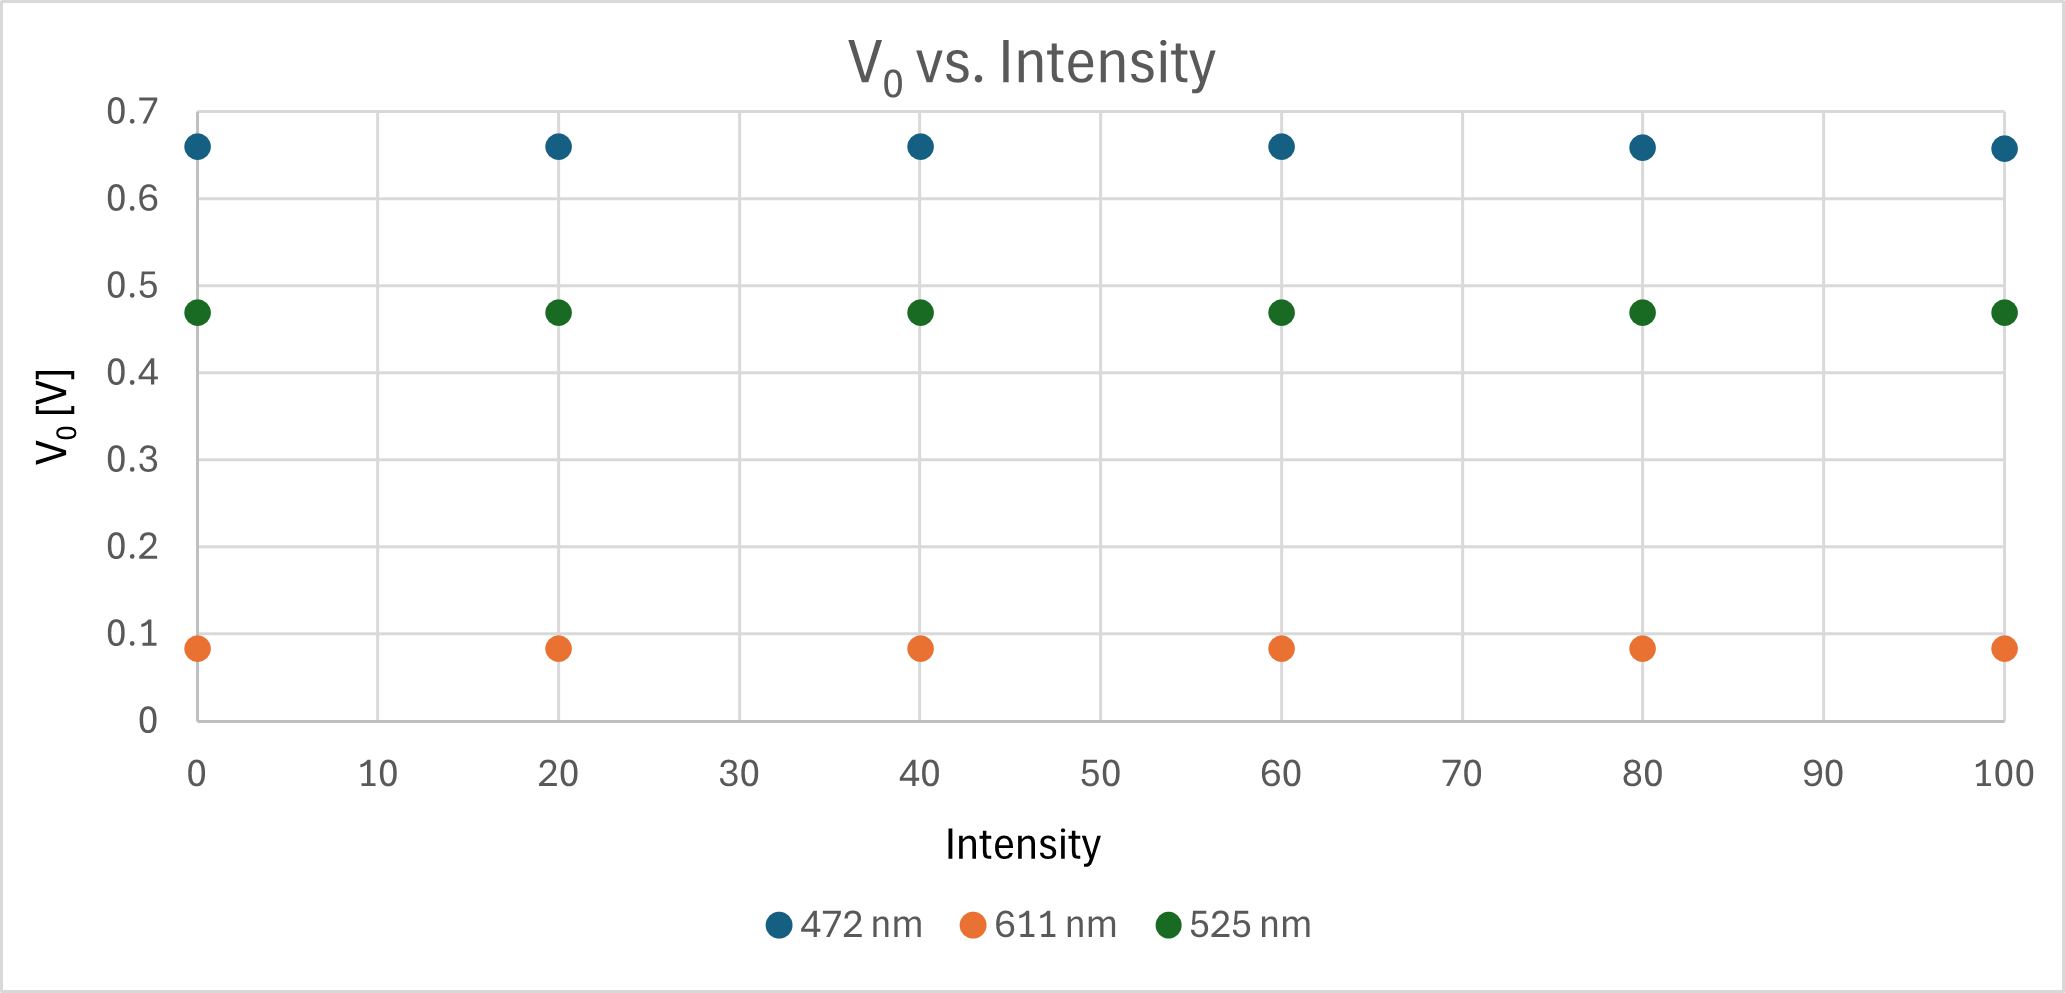
\includegraphics[width=0.8\textwidth]{V0vsIntensity}
                \caption{Graph of the V$_0$ and intensity values from table \ref{intensities}}\label{V0vsIntensities}
            \end{figure}}
            As can be seen in figure \ref{V0vsIntensities} the voltages remain constant within experimental error for every intensity. This shows that the stopping voltage does not depend on the light source's intensity and instead only on the wavelenght of the LED.
    \FloatBarrier
        \subsection{Error Analysis}
            %TODO NUMERICAL ERROR ANALYSIS
            One potential source of error comes from the design of the photoelectric tube.
            {\begin{figure}[!h]
                \centering
                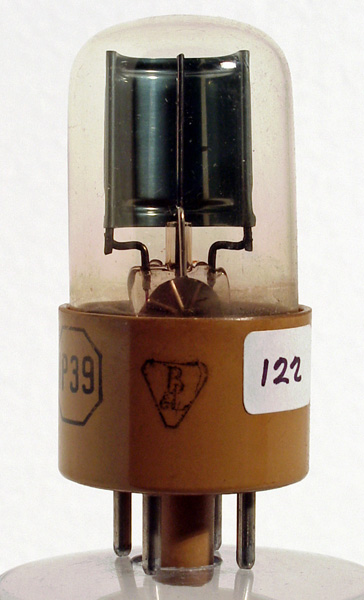
\includegraphics[width=0.25\textwidth]{1P39}
                \caption{The 1P39 photoelectric tube inside of the Planck's constant apparatus. \reference{reference:1P39PhotoelectricTube}{The Value Meuseum}{2013}}\label{1P39Image}
            \end{figure}}
            As seen in figures \ref{circuitdiagram} and \ref{1P39Image} the photoelectric tube consists of a curved photocathode with a thin anode infront of it. Depending on the format of the LED they can often be modeled as a Lambertian point emmitter \reference{reference:LEDLambertianEmitter}{Hongming Yang et al.}{2008}. Based off of this the setup can be partially simulated using an optical simulation suite. For this purpose Aether's raytracing tool Selene was used. The ray tracing setup was as follows. {\begin{figure}[!h]
                \centering
                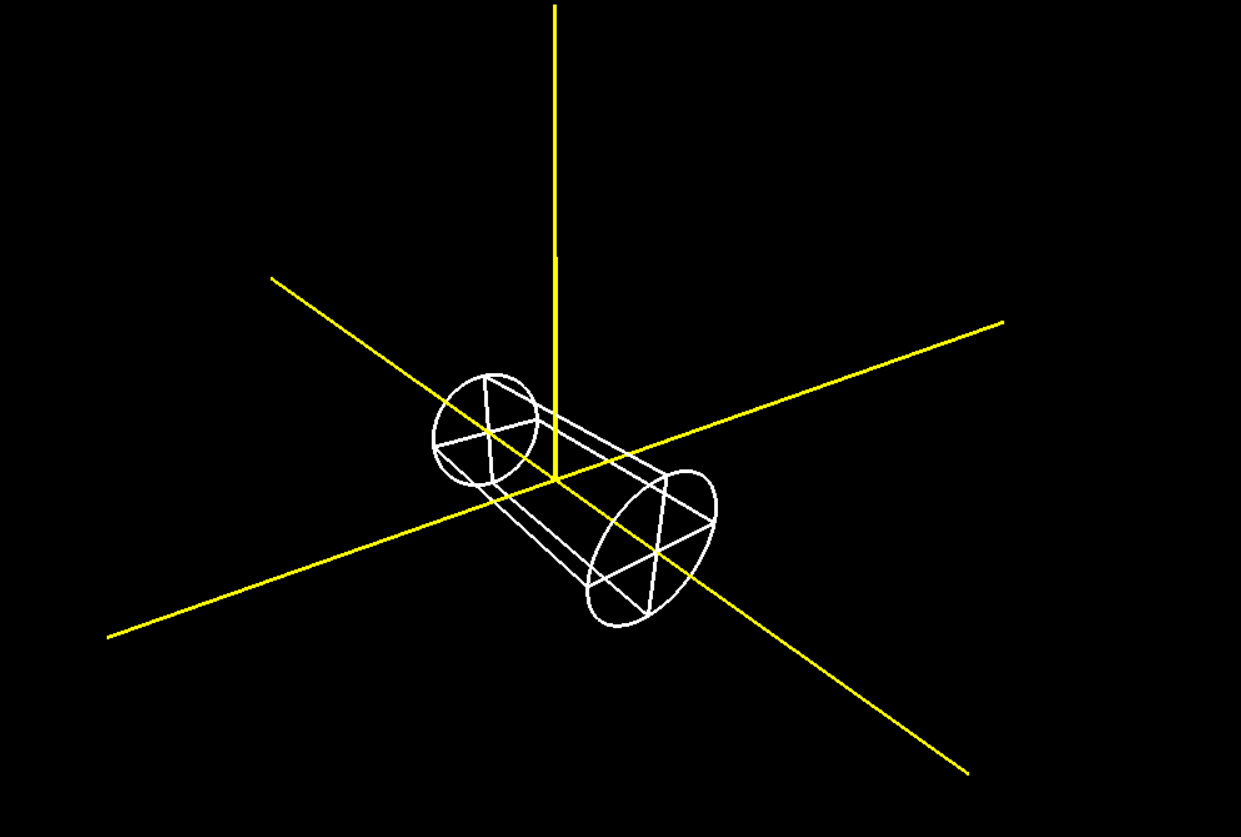
\includegraphics[width=0.5\textwidth]{aetherSimulationSetup}
                \caption{Set up within Selene.}\label{aetherSimSetup}
            \end{figure}}
            The cylinder, in white, models the photocathode. Selene is still in development so there isn't any way to model a simple, curved surface like the photocathode. To get around this the Lambertian source is placed inside the cylinder. The throw of light is $\qty{180}{\degree}$, which is not changeable. In order to not cause abberations in the later analysis stage the source was placed at the center of curvature for the surface and thus the center of the cylinder. In the real setup the source of light is beyond the center of curvature for the photocathode, however the arguments ultimately remain the same. By setting the cylinder to be act as a transparent sensor, information like ray hit distributions on it's surface could be recorded. Then, using Aether's raytracing analysis tool, the distribution of photons accross the inside of the cylinder can be found.
    \section{Discussion}
        The design of the photoelectric tube wasn't optimal for this experiment. The spread of the photons, quantified as a bell curve, adversily affected the results. This error could've been reduced by collimating the LED light, reducing the amount of spread and, thus, the experimental error. 
    \newpage
    \section{Conclusion}
        The value of Planck's constant was found to be () which conformed to the expected value of ... . 
    \addcontentsline{toc}{section}{Notes}
    \section*{Notes}
        This document was compiled using \LaTeX. Websites like Overleaf (\underline{www.overleaf.com/learn}), The TEX Stackexchange (\underline{tex.stackexchange.com}) and each package's documentation on their respective CTAN (\underline{www.ctan.org}) pages were referenced heavily for good practice and specific commands. Where possible the links to specific answers have been included in the source code as comments. The circuit diagram was made using Paul Falstad's circuit simulator (\underline{www.falstad.com/circuit}). The ray tracing simulations were done using the Aether optics simulation suite (\underline{aether.utt.fr}), specifically their ray tracer Selene and analysis programs.
    \addcontentsline{toc}{section}{References}
    %\lstinputlisting[language=Python, numbers=left, showstringspaces=false]{ep305Ass1_24365676.py}
    %REMOVE IF CODE NOT GONNA WORK
    \section*{References}
    %https://tex.stackexchange.com/questions/42905/enumerated-list-with-square-brackets
        \begin{enumerate}[label={[\arabic*]}]
            \item \label{reference:plancksConstant} General Conference on Weights and Measures, 2017, \emph{On the revision of the International System of Units (SI), Draft resolution A},s
            \uhref{https://web.archive.org/web/20180429025229/https://www.bipm.org/utils/en/pdf/CGPM/Draft-Resolution-A-EN.pdf}{www.bipm.org/utils/en/pdf/CGPM/Draft-Resolution-A-EN.pdf}, \\ archived to \uhref{https://web.archive.org/web/20180429025229/https://www.bipm.org/utils/en/pdf/CGPM/Draft-Resolution-A-EN.pdf}{web.archive.org/web/20180429025229/https://www.bip}, accessed 26/04/2026
            \item\label{reference:apparatusDocumentation} 3B Scientific, 2024, \emph{Product Manual - Planck’s Constant Apparatus - U10700-230 [1000537] (EN)}
            \item \label{reference:electronCharge} National Institute of Standards and Technology, 2022, \emph{CODATA Value: Electron Charge}, \\
            \uhref{https://physics.nist.gov/cgi-bin/cuu/Value?e}{physics.nist.gov/cgi-bin/cuu/Value?e}, accessed 20/04/2026
            \item \label{reference:speedOfLight} Bureau International des Poid et Measures, 2019, \emph{The International System of Units (SI)}, \\
            \uhref{https://www.bipm.org/en/measurement-units}{www.bipm.org/en/measurement-units}, accessed 20/04/2026
            \item \label{reference:workFunction} Lide, David R., 2008, \emph{CRC Handbook of Chemistry and Physics, 89$^{th}$ edition.}, CRC Press
            \item \label{reference:1P39PhotoelectricTube} The Valve Museum, 2013, \emph{1P39}, \uhref{https://www.r-type.org/exhib/aab0154.htm}{www.r-type.org/exhib/aab0154.htm}
            \item \label{reference:LEDLambertianEmitter} Hongming Yang, JanW. M. Bergmans, Tim C. W. Schenk, Jean-Paul M. G. Linnartz, and Ronald Rietman, 2008 \emph{An analytical model for the illuminance distribution of a power LED}, Opt. Express 16, 21641-21646
            \item \label{reference:uvPaper} Heinrich Hertz,1887, \emph{Ueber einen Einfluss des ultravioletten Lichtes auf die electrische Entladung}, Annalen der Physik 267 
        \end{enumerate}
\end{document}